\documentclass[14pt,fleqn]{extarticle}
\usepackage[T2A,T1]{fontenc}
\usepackage[utf8]{inputenc}
\usepackage[russian]{babel}
\usepackage{amsmath}
\usepackage{graphicx}
\usepackage{tabularx}
\usepackage{boldline}
\usepackage{makecell}
\usepackage{arydshln}
\usepackage{mathtools}
\usepackage{centernot}
\usepackage{enumitem}
\usepackage{nccmath}
\usepackage[a4paper, total={6.5in, 9.5in}]{geometry}

\graphicspath{ {./images/} }
\setlength{\mathindent}{0pt}
\setlength\parindent{0pt}

\def\at{
	\left.
	\vphantom{\int}
	\right|
}


\begin{document}
	\begin{titlepage}
		
\includegraphics[scale=0.12]{logo}
		\begin{center}
			\textbf{МИНОБРНАУКИ РОССИИ}\\
			\vspace{0.2cm}
			\textbf{Федеральное государственное бюджетное образовательное учреждение высшего образования}\\
			\textbf{<<САНКТ-ПЕТЕРБУРГСКИЙ ГОСУДАРСТВЕННЫЙ ЭКОНОМИЧЕСКИЙ УНИВЕРСИТЕТ>>}\\
			\vspace{0.6cm}
			Факультет информатики и прикладной математики\\
			Кафедра прикладной математики и экономико-математических методов\\
			\vspace{1cm}
			\textbf{ОТЧЁТ}\\
			по дисциплине:\\
			\textbf{<<Имитационное моделирование>>}\\
			на тему:\\
			\textbf{<<Моделирование случайных величин. Статистические испытания. Задание №2>>}\\
		\end{center}
		\vspace{1cm}
		Направление: 01.03.02\\
		Обучающийся: Бронников Егор Игоревич\\
		Группа: ПМ-1901\\
		\vfill
		\begin{center}
			Санкт-Петербург\\
			2022\\
		\end{center}
	\end{titlepage}
    \subsection*{Задание №1}
    Реализовать генератор случайных чисел, используя метод серединных квадратов (фон Нейман). Проанализировать свойства полученной последовательности.\\
    \newline

    В методе серединных квадратов изначально задаётся количество разрядов числа $k$ и начальное значение $R_0$. Далее число $R_0$ возводится в квадрат и из середины квадрата числа берётся $k$-значное число, которое снова возводится в квадрат, и так далее.\\
    Обязательным условием является то, что количество разрядов $k$ должно быть чётным числом.\\
    \newline
    Данный алгоритм был реализован на языке программирования Python. (Рисунок \ref{fig:mid_square_method_code})
    \begin{figure}[h]
        \centering 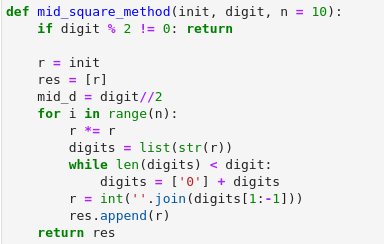
\includegraphics[scale=0.8]{mid_square_method_code}
        \caption{Реализация метода серединных квадратов}
        \label{fig:mid_square_method_code}
    \end{figure}
    \newpage
    Алгоритм был запущен с параметрами $k = 10$, $R_0 = 25$, $n = 7$, где $n$ -- это количество сгенерированных случайных чисел. Можно проследить, что при достаточно малых разрядах и малом начальном значении быстро получается вырождение, что плохо. (Рисунок \ref{fig:mid_square_method_result})
    \begin{figure}[h]
        \centering 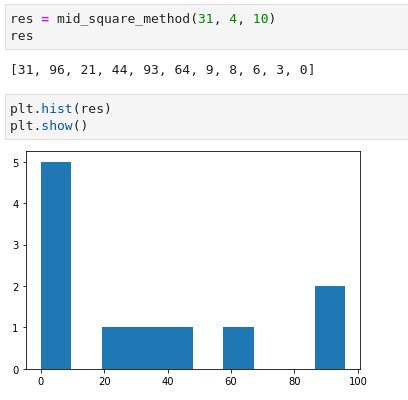
\includegraphics[scale=0.8]{mid_square_method_result}
        \caption{Результаты генерации случайных чисел методом серединных квадратов}
        \label{fig:mid_square_method_result}
    \end{figure}
    
    \subsection*{Задание №2}
    Реализовать линейный конгруэнтный датчик случайных чисел. Сгенерировать последовательность вещественных чисел, распределённых равномерно: 1) на интервале [0,1); \; 2) на интервале [a,b). Проанализировать полученные последовательности. Определить период, построить гистограмму.\\
    \newline

    Линейный конгруэнтный метод -- это один из рекуррентных методов генерации случайных чисел. Следующий элемент последовательности может быть найден по следующей формуле:
    \begin{center}
        $ r_{i+1} = (k \cdot r_i + b) \; mod \; M$
    \end{center}
    
    \newpage
    Линейная конгруэнтная последовательность, определённая числами $M$, $k$, $b$, $r_0$ периодична с периодом, не превышающим $M$. При этом длина периода равна $M$ тогда и только тогда, когда:
    \begin{enumerate}[topsep=0pt,itemsep=-1ex,partopsep=1ex,parsep=1ex]
        \item числа $b$ и $M$ взаимно простые;
        \item $k-1$ кратно $p$ для каждого простого $p$, являющегося делителем $M$;
        \item $k-1$ кратно 4, если $M$ кратно 4.
    \end{enumerate}
    Сначала был реализован алгоритм для интервала [0;1) на языке программирования Python. (Рисунок \ref{fig:linear_congruent_gauge_0_1_code})
    \begin{figure}[h]
        \centering 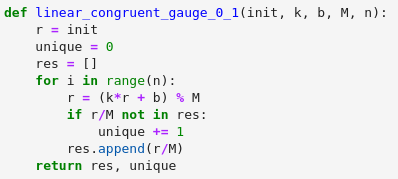
\includegraphics[scale=0.8]{linear_congruent_gauge_0_1_code}
        \caption{Реализация линейного конгруэнтного счётчика на интервале [0,1)}
        \label{fig:linear_congruent_gauge_0_1_code}
    \end{figure}

    Для того чтобы получить случайные числа в интервале от [0,1) нужно поделить каждый случайный сгенерированный элемент последовательности на $M$. Также данная функция выводит период сгенерированной последовательности.
    \begin{figure}[h]
        \centering 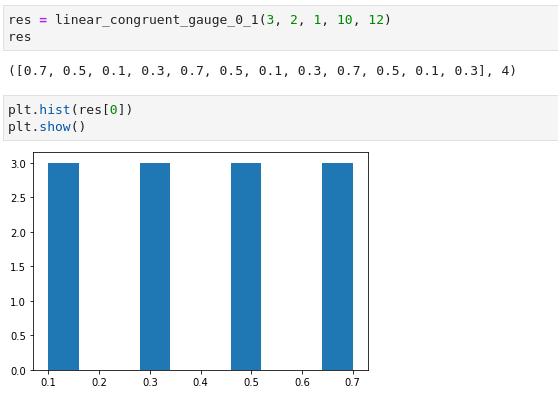
\includegraphics[scale=0.52]{linear_congruent_gauge_0_1_result}
        \caption{Результаты генерации случайных чисел линейным конгруэнтным счётчиком на интервале [0,1)}
        \label{fig:linear_congruent_gauge_0_1_result}
    \end{figure}
    \newpage
    В качестве аргументов были выбраны следующие значения: $r_0 = 3$, $k = 2$, $b = 1$, $M = 10$, $n = 12$, где $n$ -- это количество сгенерированных случайных чисел. Можно видеть, что при данном наборе аргументов длина периода составила 4. (Рисунок \ref{fig:linear_congruent_gauge_0_1_result})\\
    \newline
    Далее был реализован алгоритм для интервала [a;b). (Рисунок \ref{fig:linear_congruent_gauge_a_b_code})
    \begin{figure}[h]
        \centering 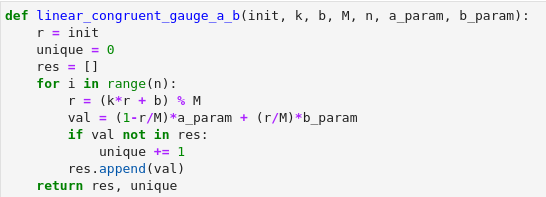
\includegraphics[scale=0.6]{linear_congruent_gauge_a_b_code}
        \caption{Реализация линейного конгруэнтного счётчика на интервале [a,b)}
        \label{fig:linear_congruent_gauge_a_b_code}
    \end{figure}

	Для того чтобы получить случайные числа в интервале от [a,b) нужно проделать следующее преобразование:
	\begin{center}
		$(1 - \dfrac{r_i}{M})/a + \dfrac{r_i}{M} \cdot b$
	\end{center}
	То есть сначала мы генерируем числа в интервале от [0,1), а дальше преобразуем их к интервалу от [a,b).
 	\begin{figure}[h]
		\centering 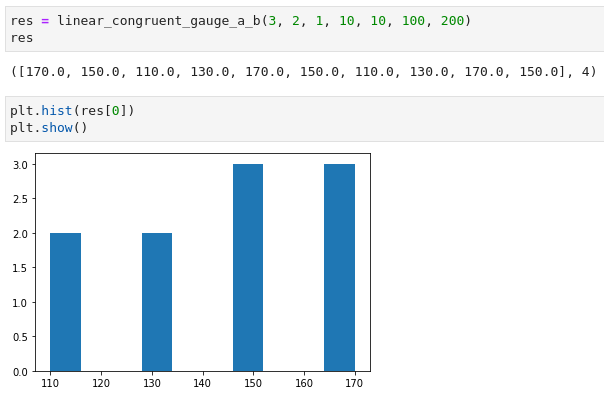
\includegraphics[scale=0.52]{linear_congruent_gauge_a_b_result}
		\caption{Результаты генерации случайных чисел линейным конгруэнтным счётчиком на интервале [a,b)}
		\label{fig:linear_congruent_gauge_a_b_result}
	\end{figure}
    \newpage
	В качестве аргументов были выбраны следующие значения: $r_0 = 3$, $k = 2$, $b = 1$, $M = 10$, $n = 10$, $a_{param} = 100$, $b_{param} = 200$, где $n$ -- это количество сгенерированных случайных чисел. Можно видеть, что при данном наборе аргументов длина периода составила 4. (Рисунок \ref{fig:linear_congruent_gauge_a_b_result})\\
	
	\subsection*{Задание №3}
	Используя метод обратной функции, получить последовательность случайных чисел, распределённых экспоненциально с заданным параметром $\lambda$. Проанализировать полученную последовательность. Оценить математическое ожидание  и дисперсию, построить гистограмму.\\
	\newline
	
	Плотность распределения экспоненциального закона:
	\begin{ceqn}
	\begin{align*}
		f(x) =
		\begin{cases}
			\lambda e^{-\lambda \cdot x} \quad x \geq 0\\
			0 \hspace{1.55cm} x < 0
		\end{cases}
	\end{align*}
	\end{ceqn}

	Функция распределения экспоненциального закона:
	\begin{ceqn}
	\begin{align*}
		F(x) =
		\begin{cases}
			1 - e^{-\lambda \cdot x} \quad x \geq 0\\
			0 \hspace{2.15cm} x < 0
		\end{cases}
	\end{align*}
	\end{ceqn}

	Получается, что обратная функция $F^{-1}(x)$ будет выглядеть следующим образом:
	\begin{center}
		$x = \dfrac{-ln(1-y)}{\lambda} = -\dfrac{ln(y)}{\lambda}$
	\end{center}
	Если подставлять вместо $y$ случайные равномерно распределённые значения, то можно получать требуемые числа.
	\newpage
	Таким образом, была реализована функция на языке программирования Python. (Рисунок \ref{fig:exp_inverse_function_method_code})
	\begin{figure}[h]
		\centering 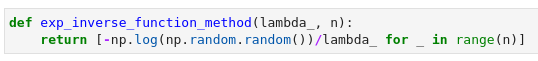
\includegraphics[scale=0.8]{exp_inverse_function_method_code}
		\caption{Реализация метода обратной функции для экспоненциального закона}
		\label{fig:exp_inverse_function_method_code}
	\end{figure}

		При $\lambda = 3$ и $n = 1000$ получается следующий результат. (Рисунок \ref{fig:exp_inverse_function_method_result})
	\begin{figure}[h]
		\centering 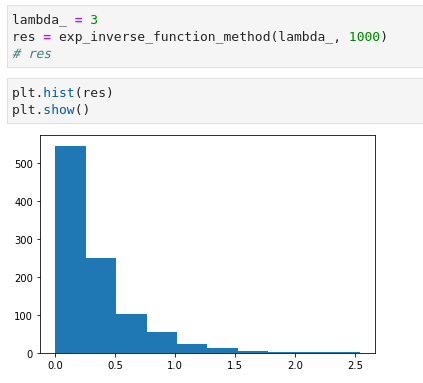
\includegraphics[scale=0.8]{exp_inverse_function_method_result}
		\caption{Результаты генерации случайных чисел методом обратной функции для экспоненциального закона}
		\label{fig:exp_inverse_function_method_result}
	\end{figure}

	Математическое ожидание экспоненциального распределения:
	\begin{ceqn}
		\begin{align*}
			E = \dfrac{1}{\lambda}
		\end{align*}
	\end{ceqn}
	\newpage
	Если рассчитывать математическое ожидание как среднее значение в выборке, то получается следующий результат. (Рисунок \ref{fig:exp_inverse_function_method_math})
	\begin{figure}[h]
		\centering 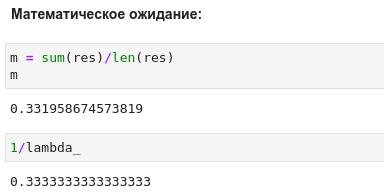
\includegraphics[scale=0.7]{exp_inverse_function_method_math}
		\caption{Теоретическое и расчётное значения математического ожидания ($\lambda = 3$)}
		\label{fig:exp_inverse_function_method_math}
	\end{figure}

	Можно заметить, что при $n = 1000$ значения получились достаточно близкими.\\
	Дисперсия экспоненциального распределения:
	\begin{ceqn}
		\begin{align*}
			D = \dfrac{1}{\lambda^2}
		\end{align*}
	\end{ceqn}
	Далее можно рассчитать дисперсию как среднее квадратное отклонение от среднего значения выборки. (Рисунок \ref{fig:exp_inverse_function_method_var})
	\begin{figure}[h]
		\centering 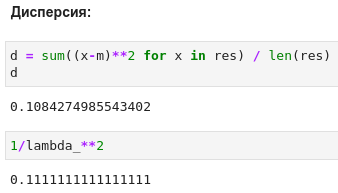
\includegraphics[scale=0.7]{exp_inverse_function_method_var}
		\caption{Теоретическое и расчётное значения дисперсии ($\lambda = 3$)}
		\label{fig:exp_inverse_function_method_var}
	\end{figure}

	Можно заметить, что при $n = 1000$ значения получились достаточно близкими.
	
	\newpage
	\subsection*{Задание №4}
	Для треугольного распределения получить функцию распределения. Используя метод обратной функции, получить последовательность случайных чисел с треугольным распределением. Оценить математическое ожидание и дисперсию, построить гистограмму.\\
	\newline
	
	Пусть имеются следующие параметры: $a$ (\textit{min}), $b$ (\textit{max}), $c$ (\textit{мода}).\\
    Плотность треугольного распределения:
    \begin{ceqn}
	\begin{align*}
		f(x) =
		\begin{cases}
			\dfrac{2(x-a)}{(b-a)(c-a)} \quad , x \in [a,c]\\
			\dfrac{2(b-x)}{(b-c)(b-a)} \quad , x \in [c,b]\\
			0 \hspace{3.25cm} , x \centernot\in [a,b]\\
		\end{cases}
	\end{align*}
    \end{ceqn}

    Функция распределения треугольного закона:
    \begin{ceqn}
	\begin{align*}
		F(x) =
		\begin{cases}
			0 \hspace{4.1cm} , x < a\\
			\dfrac{(x-a)^2}{(b-a)(c-a)} \hspace{1.3cm} , x \in [a,c]\\
			1 - \dfrac{(x-b)^2}{(b-a)(b-c)} \quad , x \in [c,b]\\
			1 \hspace{4.1cm} , x > b\\
		\end{cases}
	\end{align*}
    \end{ceqn}

	Получается, что обратная функция $F^{-1}(x)$ будет выглядеть следующим образом:
	\begin{ceqn}
	\begin{align*}
		F^{-1}(y) = x =
		\begin{cases}
			a + \sqrt{(b-a)(c-a)y} \hspace{2.2cm} , 0 < y < \dfrac{c-a}{b-a}\\
			b - \sqrt{(b-a)(b-c)(1-y)} \hspace{1cm} , \dfrac{c-a}{b-a} \leq y < 1\\
		\end{cases}
	\end{align*}
    \end{ceqn}

	Если подставить вместо $y$ случайные равномерно распределённые значения, то можно получить требуемые числа.
	\newpage
	Таким образом, была реализована функция на языке программирования Python. (Рисунок \ref{fig:triangle_inverse_function_method_code})
	\begin{figure}[h]
		\centering 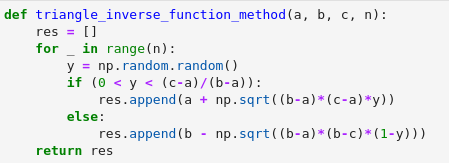
\includegraphics[scale=0.7]{triangle_inverse_function_method_code}
		\caption{Реализация метода обратной функции для треугольного закона}
		\label{fig:triangle_inverse_function_method_code}
	\end{figure}

	При $a = 0$, $b = 1$, $c = 0.5$ и $n = 10$ получается следующий результат. (Рисунок \ref{fig:triangle_inverse_function_method_result})
	\begin{figure}[h]
		\centering 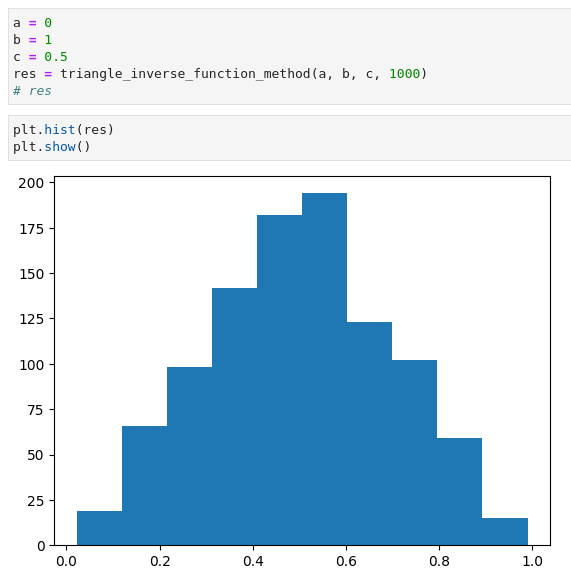
\includegraphics[scale=0.5]{triangle_inverse_function_method_result}
		\caption{Результаты генерации случайных чисел методом обратной функции для треугольного закона}
		\label{fig:triangle_inverse_function_method_result}
	\end{figure}
	
	Математическое ожидание треугольного распределения:
	\begin{ceqn}
	\begin{align*}
		E = \dfrac{a + b + c}{3}
	\end{align*}
	\end{ceqn}
	\newpage
	Если рассчитывать математическое ожидание как среднее значение в выборке, то получается следующий результат. (Рисунок \ref{fig:triangle_inverse_function_method_math})
	\begin{figure}[h]
		\centering 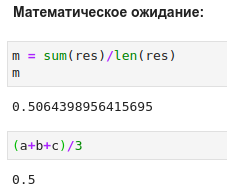
\includegraphics[scale=0.7]{triangle_inverse_function_method_math}
		\caption{Теоретическое и расчётное значения математического ожидания ($a = 0$, $b = 1$, $c = 0.5$)}
		\label{fig:triangle_inverse_function_method_math}
	\end{figure}
	
	Можно заметить, что при $n = 1000$ значения получились достаточно близкими.\\
	Дисперсия треугольного распределения:
	\begin{ceqn}
		\begin{align*}
			D = \dfrac{a^2 + b^2 +c^2 - a \cdot b - a \cdot c - b \cdot c}{18}
		\end{align*}
	\end{ceqn}
	Далее можно рассчитать дисперсию как среднее квадратное отклонение от среднего значения выборки. (Рисунок \ref{fig:triangle_inverse_function_method_var})
	\begin{figure}[h]
		\centering 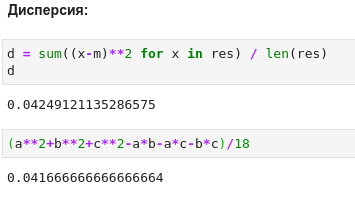
\includegraphics[scale=0.7]{triangle_inverse_function_method_var}
		\caption{Теоретическое и расчётное значения дисперсии ($a = 0$, $b = 1$, $c = 0.5$)}
		\label{fig:triangle_inverse_function_method_var}
	\end{figure}
	
	Можно заметить, что при $n = 1000$ значения получились достаточно близкими.
	
	\newpage
	
	\subsection*{Задание №5}
	Получить нормально распределённую последовательность случайных чисел, используя:
	\begin{enumerate}[topsep=0pt,itemsep=-1ex,partopsep=1ex,parsep=1ex]
		\item преобразование Бокса-Мюллера
		\item формулу $Z = \sqrt{\dfrac{12}{n}}\left(\smashoperator[r]{\sum_{i=1}^{n}} x_i - \dfrac{n}{2}\right)$ (частный случай $Z = \smashoperator[r]{\sum_{i=1}^{12}} x_i - 6$)
	\end{enumerate}

	\vspace{1cm}
	
	\textit{1. Преобразование Бокса-Мюллера}\\

	Данное преобразование заключается в замене равномерно распределённых случайных величин на нормально распределённые случайные величины, которые можно найти по следующим формулам:
	\begin{ceqn}
	\begin{align*}
		u_1 = \cos(2 \pi \cdot v_1) \sqrt{-2 \cdot \ln(v_2)}\\
		u_2 = \sin(2 \pi \cdot v_1) \sqrt{-2 \cdot \ln(v_2)}
	\end{align*}
	\end{ceqn}
	То есть на каждом шаге создания нового элемента последовательности нужно сначала сгенерировать два равномерно распределённых случайных числа $v_1$ и $v_2$, а дальше случайно выбрать формулу $u_1$ или $u_2$ для расчёта результирующего элемента последовательности.\\
	
	
	Данный алгоритм был реализован на языке программирования Python. (Рисунок \ref{fig:box_muller_transform_code})
	\begin{figure}[h]
		\centering 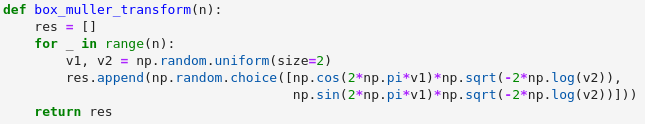
\includegraphics[scale=0.65]{box_muller_transform_code}
		\caption{Реализация преобразования Бокса-Мюллера}
		\label{fig:box_muller_transform_code}
	\end{figure}
	
	\newpage
	Была сгенерирована последовательность из 1000 элементов и на основании этого построена гистограмма. (Рисунок \ref{fig:box_muller_transform_result})

	\begin{figure}[h]
		\centering 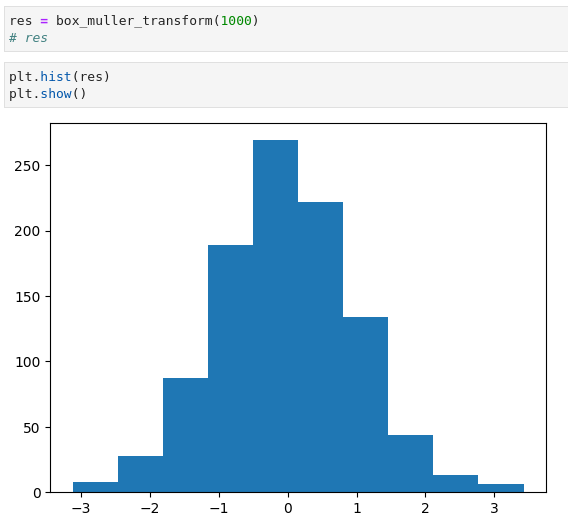
\includegraphics[scale=0.6]{box_muller_transform_result}
		\caption{Результаты применения преобразования Бокса-Мюллера}
		\label{fig:box_muller_transform_result}
	\end{figure}
	
	Как можно видеть на получившейся гистограмме, распределение действительно получилось нормальное, то есть алгоритм сработал корректно.
	
	\vspace{1cm}
	
	\textit{2. Применение центральной предельной теоремы}\\
	
	В данном алгоритме нужно изначально сгенерировать $n$ штук случайных равномерных чисел и дальше воспользоваться формулой, которая вытекает из центральной предельной теоремы:
	\begin{ceqn}
	\begin{align*}
		Z = \sqrt{\dfrac{12}{n}}\left(\smashoperator[r]{\sum_{i=1}^{n}} x_i - \dfrac{n}{2}\right)
	\end{align*}
	\end{ceqn}

	\newpage
	
	Данный алгоритм был реализован на языке программирования Python. (Рисунок \ref{fig:central_limit_theorem_code})
	\begin{figure}[h]
		\centering 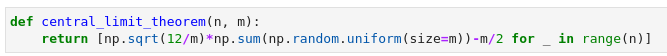
\includegraphics[scale=0.65]{central_limit_theorem_code}
		\caption{Реализация применения центральной предельной теоремы}
		\label{fig:central_limit_theorem_code}
	\end{figure}
	
	Была сгенерирована последовательность из 1000 элементов и на основании этого построена гистограмма. (Рисунок \ref{fig:central_limit_theorem_result})
	
	\begin{figure}[h]
		\centering 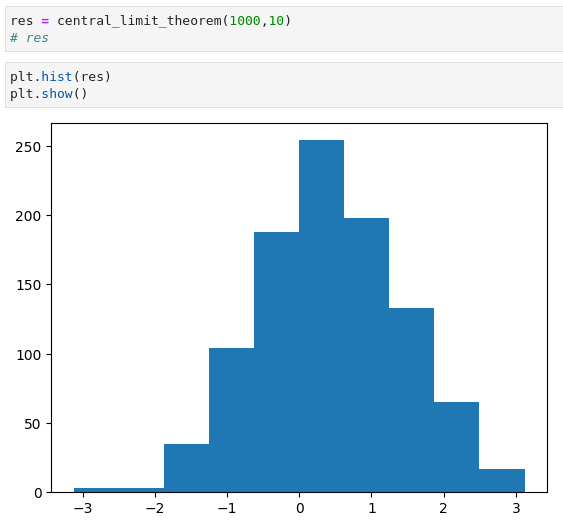
\includegraphics[scale=0.6]{central_limit_theorem_result}
		\caption{Результаты применения центральной предельной теоремы}
		\label{fig:central_limit_theorem_result}
	\end{figure}
	
	Как можно видеть на получившейся гистограмме, распределение действительно получилось нормальное, то есть алгоритм сработал корректно.
	
	\newpage
	
	\subsection*{Задание №6}
	Используя метод Монте-Карло, вычислить $\int_{0}^{1} \sin(\pi x) dx$. Проанализируйте, как зависит точность полученного результата от количества точек, использованных для получения оценки. Постройте график этой зависимости.
	\newline
	
	Для начала стоить нарисовать график данной функции $\sin (\pi x)$ и сгенерировать $n$ штук случайных точек.  (Рисунок \ref{fig:monte_carlo_example})
	\begin{figure}[h]
		\centering 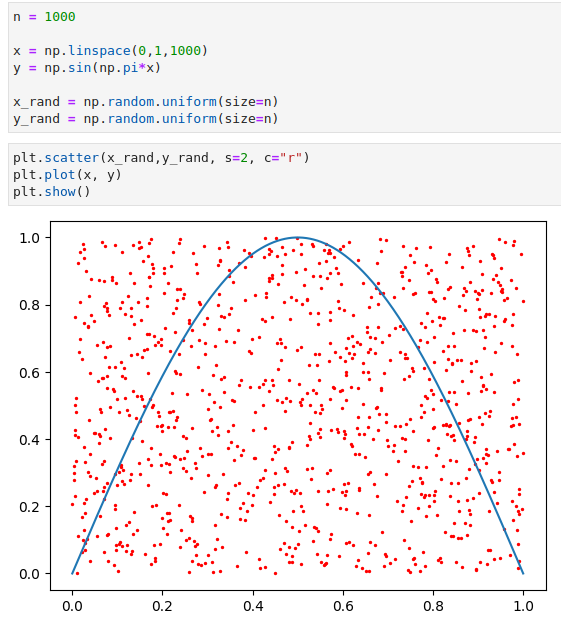
\includegraphics[scale=0.6]{monte_carlo_example}
		\caption{Пример применения метода Монте-Карло}
		\label{fig:monte_carlo_example}
	\end{figure}
	
	Далее остаётся просто посчитать то количество точек, которые попали под график и разделить их на общее количество сгенерированных точек.
	
	\newpage
	
	Данный алгоритм был реализован на языке программирования Python. (Рисунок \ref{fig:monte_carlo_code})
	\begin{figure}[h]
		\centering 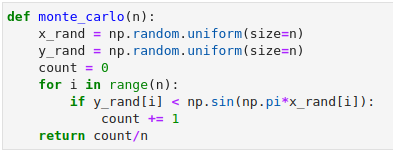
\includegraphics[scale=0.65]{monte_carlo_code}
		\caption{Реализация метода Монте-Карло для подсчёта интеграла}
		\label{fig:monte_carlo_code}
	\end{figure}

	Также была проанализирована зависимость между точностью результата и количеством сгенерированных точек. (Рисунок \ref{fig:monte_carlo_result})
	\begin{figure}[h]
		\centering 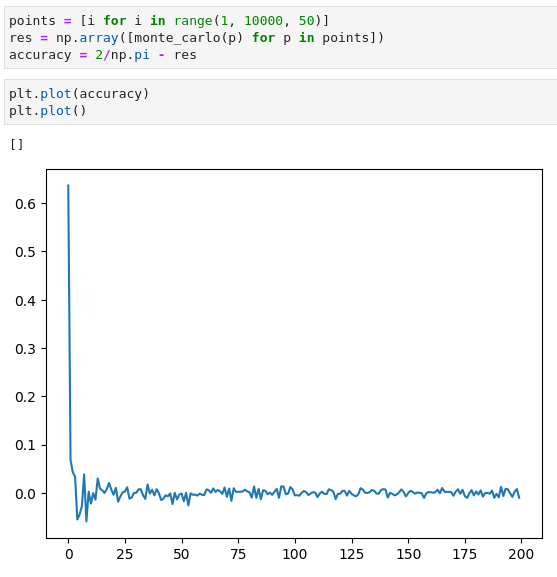
\includegraphics[scale=0.5]{monte_carlo_result}
		\caption{Зависимость точности результатов от количества точек}
		\label{fig:monte_carlo_result}
	\end{figure}

	Как можно видеть на графике, что чем больше количество сгенерированных точек, то тем точнее получается результат.
	
	\newpage
	
	\subsection*{Задание №7}
	Используя метод статистических испытаний, оценить вероятность выпадения герба при бросании правильной монеты. Проанализируйте, как зависит точность полученного результата от количества точек, использованных для получения оценки. Постройте график этой зависимости.
	\newline
	
	Для решения данной задачи стоить сгенерировать $n$ случайных равномерно распределённых чисел, если $x_i < 0.5$, то добавлять в результирующий список 0, в противном случае 1. Далее стоит просуммировать элементы получившегося списка и разделить на количество элементов в этом списке.\\
	
	Данный алгоритм был реализован на языке программирования Python. (Рисунок \ref{fig:coin_code})
	\begin{figure}[h]
		\centering 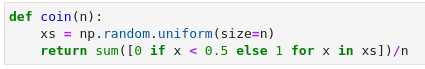
\includegraphics[scale=0.65]{coin_code}
		\caption{Реализация метода статистических испытаний}
		\label{fig:coin_code}
	\end{figure}

	Также была проанализирована зависимость между точностью результата и количеством сгенерированных точек. (Рисунок \ref{fig:coin_result})
	\begin{figure}[h]
		\centering 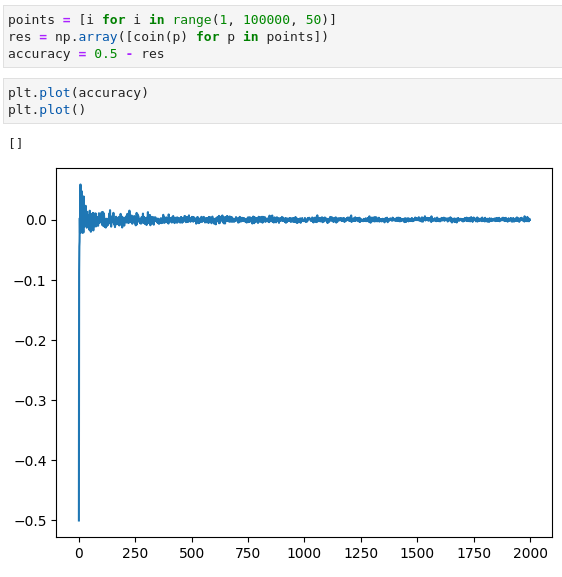
\includegraphics[scale=0.4]{coin_result}
		\caption{Зависимость точности результатов от количества точек}
		\label{fig:coin_result}
	\end{figure}

	Как можно видеть на графике, что чем больше количество сгенерированных точек, то тем точнее получается результат.
\end{document}
